\chapter{Organisational Risk Assessment}\label{ch:organisational-risk-assessment}
In this chapter, an organisational risk management plan will be made in order to assess and manage the relevant risks to the project.
In order to realise this risk management plan, a SWOT diagram is displayed and abbreviated on in \cref{sec:SWOT-Analysis}.
This diagram will be used as the input for the risk analysis in \cref{sec:Risk-Analysis}.


\section{SWOT Analysis}\label{sec:SWOT-Analysis}
A SWOT analysis is a planning tool that helps identify the Strengths and Weaknesses, which are internal aspects, and Opportunities and Threats, which are external aspects involved in the organisation.
In \cref{fig:swotanalysis} the SWOT diagram can be seen.
\begin{figure}[ht]
    \centering
    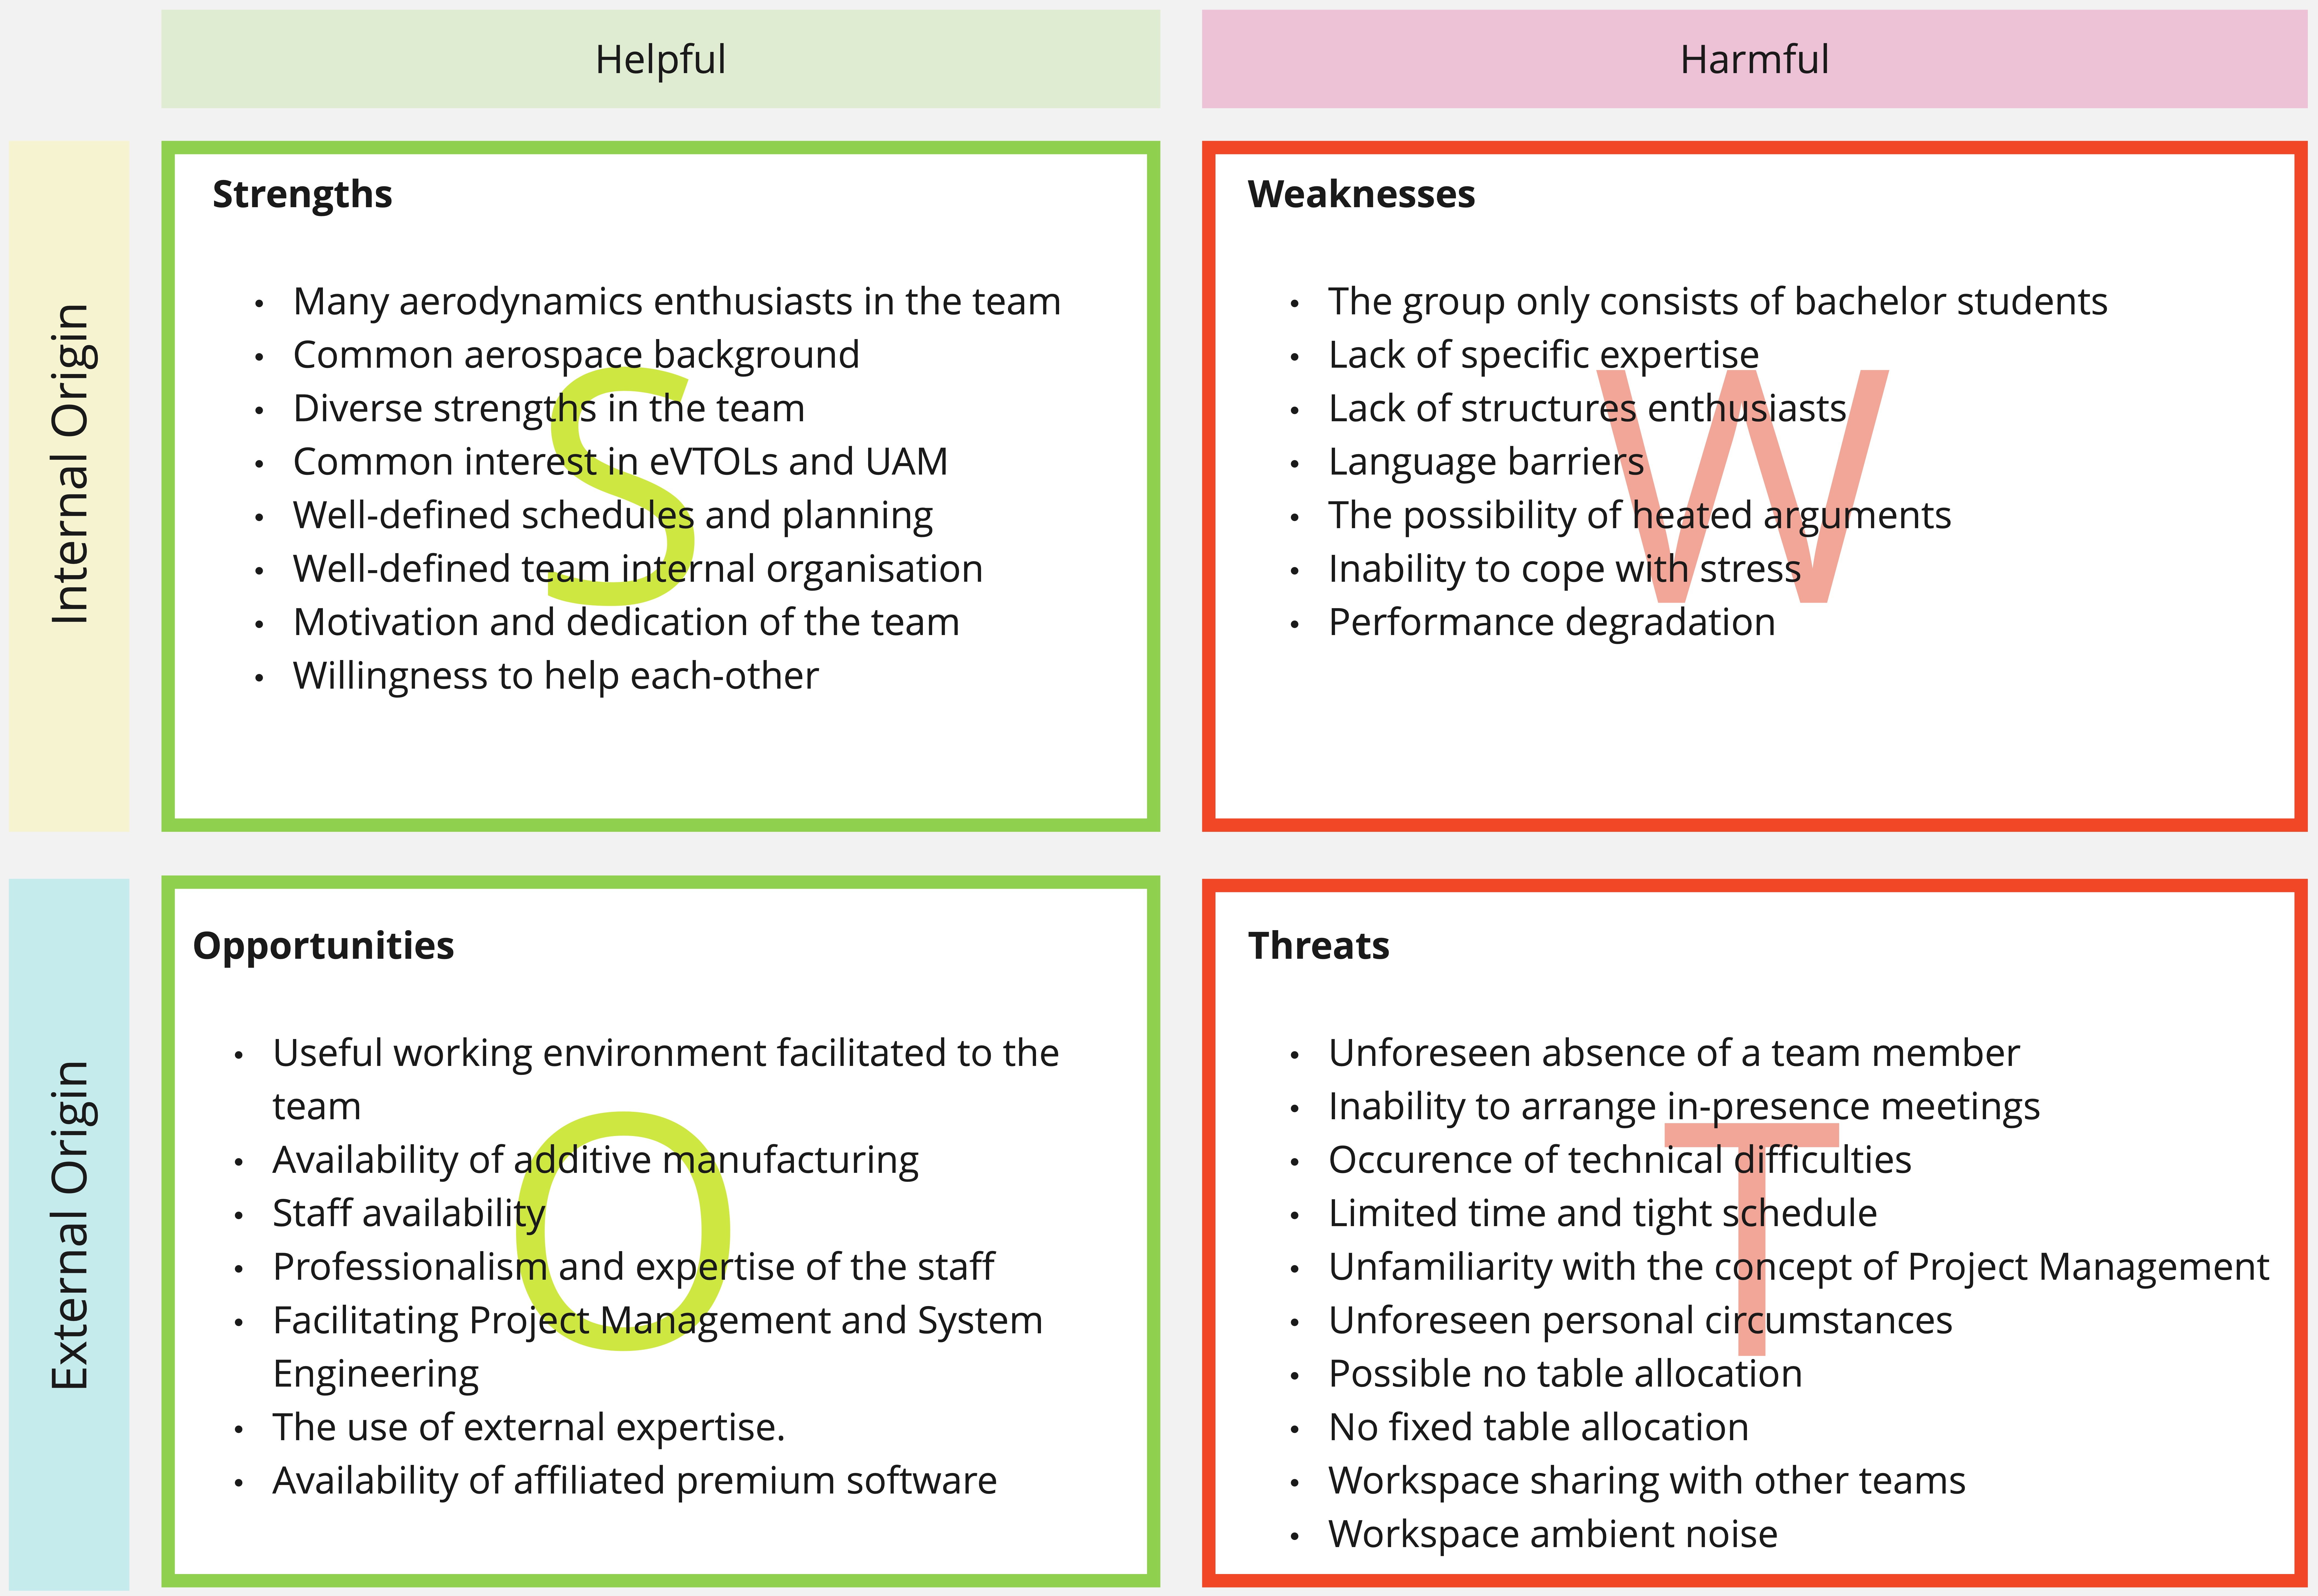
\includegraphics[width=\linewidth]{figures/Copy SWOT Analysis.jpg}
    \caption{SWOT Diagram}
    \label{fig:swotanalysis}
\end{figure}

This analysis is used to understand and identify potential organisational risks.
If a weakness is a threat as well, this is considered a serious risk, because an external threat induces problems.
If this is a team weakness, however, problems might arise if proper risk mitigation is not executed.


\section{Risk Analysis}\label{sec:Risk-Analysis}
This section presents the results of the risk analysis.
Firstly, in \cref{subsec:Risk-Metrics} the most important risks are identified, utilising the SWOT analysis.
During this analysis, the likelihood and the scheduled impact of the risk are determined, which will result in a final score.
Next, the risk register and map are constructed in \cref{subsec:Risk-Register-and-Map} to assist risk mitigation and contingency planning.
Thereafter, the mitigation strategy and contingency plan are proposed in \cref{subsec:Risk-Mitigation-and-Contingency-Plan} to decrease the likelihood and impact of the risk.
Finally, the mitigated risk register and map are presented in \cref{tab:mitriskregister,fig:riskmaps}.

\subsection{Risk Metrics}\label{subsec:Risk-Metrics}
Before the risk events can be identified and quantified a metrics system shall be defined.
A risk event has two distinguishable properties, the likelihood and the impact of an event on the project.
These two properties are quantified on a scale range of 1 to 5.
The description of the two metrics are summarised in \cref{tab:likelihood_metrics,tab:impact_metrics}.

\begin{table}[ht]
    \centering

    \begin{minipage}{0.5\textwidth}
        \centering
        \begin{tabular}{ccc}
            \hline
            Likelihood & Description & Probability         \\ \hline
            5          & Very High   & $0.7\leq P$         \\
            4          & High        & $ 0.5 \leq P < 0.7$ \\
            3          & Moderate    & $0.3 \leq P < 0.5$  \\
            2          & Low         & $0.05 \leq P < 0.3$ \\
            1          & Very Low    & $P < 0.05$          \\ \hline
        \end{tabular}
        \caption{Likelihood metrics}
        \label{tab:likelihood_metrics}
    \end{minipage}\hfill
    \begin{minipage}{0.5\textwidth}
        \centering
        \begin{tabular}{cc}
            \hline
            Impact & Description  \\ \hline
            5      & Catastrophic \\
            4      & Critical     \\
            3      & Marginal     \\
            2      & Acceptable   \\
            1      & Negligible   \\ \hline
        \end{tabular}
        \caption{Impact metrics}
        \label{tab:impact_metrics}
    \end{minipage}
\end{table}

\subsection{Risk Register and Map}\label{subsec:Risk-Register-and-Map}
An efficient way of risk identification and handling is the generation of a risk register and map.
The investigation of the risk events employed the results of the SWOT analysis in \cref{sec:SWOT-Analysis}. Different phases of the project were considered to identify the major risk events.
For each phase, several planning risk categories were recognised.
These entail: organizational, schedule, communication, internal, external and resource.
All categories were broken down into several risk events. Subsequently, the impacts were described and quantified alongside the likelihood.
Finally, the risk was quantified as the product of the normalised likelihood and the impact.
The resulting risk register of the risk investigation is depicted in \cref{tab:mitriskregister}.

All the unmitigated risks stated in \cref{tab:unmitigated_risk_map}, can be plotted into a risk map, which can be seen in \cref{fig:unmitigated}.
The map visualizes the severity of the risk and gives an easy overview of which risks need to be mitigated.
For example, it can be seen that R-G-6 and R-G-7 require a mitigation strategy, because they are positioned in the red top-right zone of \cref{fig:unmitigated}.
\begin{table}[ht]
\caption{Unmitigated organizational risk register}
    \label{tab:unmitigated_risk_map}
    \centering
    \resizebox{\linewidth}{!}{
        \begin{tabular}{lclllccc}
            \hline
            \multicolumn{1}{c}{\multirow{2}{*}{Risk ID}} & \multirow{2}{*}{Period} & \multicolumn{1}{c}{\multirow{2}{*}{Category}}                    & \multicolumn{1}{c}{\multirow{2}{*}{Risk Description}}                                                           & \multicolumn{1}{c}{\multirow{2}{*}{Impact Description}}                                     & \multicolumn{3}{c}{Unmitigated Risk}                                               \\
            \cline{6-8}
            \multicolumn{1}{c}{} & & \multicolumn{1}{c}{} & \multicolumn{1}{c}{}                 & \multicolumn{1}{c}{}                                                                        & \multicolumn{1}{l}{Likelihood} & Impact & Risk                                     \\ \hline
            R-G-1 & \multirow{8}{*}{All} & Schedule & \begin{tabular}[c]{@{}l@{}}
                                                          Incorrect time allocation, \\insufficient time is given for tasks
            \end{tabular} & Accumulated Delays & 4 & 4 & {\cellcolor[rgb]{0.502,0.541,0.533}}3.2 \\
            R-G-2 & & Schedule & Unforeseen absence of a team member & \begin{tabular}[c]{@{}l@{}}
                                                                           Decreased working\\capacity
            \end{tabular}                & 2 & 5             & {\cellcolor[rgb]{0.545,0.776,0.471}}2    \\
            R-G-3                & & Schedule             & interdependencies of tasks~ & \begin{tabular}[c]{@{}l@{}}
                                                                                              Decreased working \\efficiency\\and increased time~
            \end{tabular} & 5 & 3 & {\cellcolor[rgb]{0.51,0.58,0.522}}3 \\
            R-G-4                & & External        & Unavailability of tutors, coaches          & Increased uncertainity & 2                              & 3      & {\cellcolor[rgb]{0.239,0.898,0.714}}1.2   \\
            R-G-5 & & External & Unavailability of~ teacher assistant & Increased uncertainity & 1 & 2 & {\cellcolor[rgb]{0.082,0.922,0.843}}0.4 \\
            R-G-6 & & Schedule & \begin{tabular}[c]{@{}l@{}}
                                     Inability to arrange in-presence \\meetings when no table is available
            \end{tabular} & \begin{tabular}[c]{@{}l@{}}
                                Decreased communication\\and working~efficiency
            \end{tabular} & 4 & 5 & {\cellcolor[rgb]{0.475,0.384,0.573}}4 \\
            R-G-7 & & Communication & \begin{tabular}[c]{@{}l@{}}
                                          Inadequate communication\\~between team members and roles
            \end{tabular} & \begin{tabular}[c]{@{}l@{}}
                                Working parallel on\\the same task
            \end{tabular} & 4 & 5 & {\cellcolor[rgb]{0.475,0.384,0.573}}4 \\
            R-G-8 & & Communication & Working space distractions~ & Decreased work quality & 5 & 1 & {\cellcolor[rgb]{0.082,0.922,0.843}}1 \\ \hline
            R-P-1 & \multirow{4}{*}{\begin{tabular}[c]{@{}c@{}}
                                        Project\\Planning
            \end{tabular}} & Internal & Unfamiliarity with Project Management & \begin{tabular}[c]{@{}l@{}}
                                                                                    Slow project planning\\progress
            \end{tabular} & 3 & 4 & {\cellcolor[rgb]{0.529,0.698,0.49}}2.4 \\
            R-P-2 & & Internal & Lack of all needed range of expertise & \begin{tabular}[c]{@{}l@{}}
                                                                             Decreased personal\\motivation
            \end{tabular} & 5 & 3 & {\cellcolor[rgb]{0.51,0.58,0.522}}3 \\
            R-P-3 & & Organizational & \begin{tabular}[c]{@{}l@{}}
                                           Unimplemented risk mitigation\\by the responsible members
            \end{tabular} & Unsupervised risks & 3 & 5 & {\cellcolor[rgb]{0.51,0.58,0.522}}3 \\
            R-P-4 & & Organizational & \begin{tabular}[c]{@{}l@{}}
                                           Excessive expectations are set \\during project planning
            \end{tabular} & Accumulated Delays & 4 & 3 & {\cellcolor[rgb]{0.529,0.698,0.49}}2.4 \\ \hline
            R-C-1 & \begin{tabular}[c]{@{}c@{}}
                        Conceptual\\~phase
            \end{tabular} & Schedule & \begin{tabular}[c]{@{}l@{}}
                                           Unable to come up with sufficient \\number of feasible concepts
            \end{tabular} & \begin{tabular}[c]{@{}l@{}}
                                Less optimal solution\\outcome
            \end{tabular} & 3 & 2 & {\cellcolor[rgb]{0.239,0.902,0.714}}1.2 \\ \hline
            R-T-1 & \begin{tabular}[c]{@{}c@{}}
                        Trade-off \\Phase
            \end{tabular} & Schedule & \begin{tabular}[c]{@{}l@{}}
                                           Unable to complete the trade-off\\and conclude the final design concept
            \end{tabular} & \begin{tabular}[c]{@{}l@{}}
                                Delay in preliminary and\\detailed design
            \end{tabular} & 2 & 5 & {\cellcolor[rgb]{0.545,0.776,0.471}}2 \\ \hline
            R-PD-1 & \begin{tabular}[c]{@{}c@{}}
                         Preliminary\\Design
            \end{tabular} & Schedule & \begin{tabular}[c]{@{}l@{}}
                                           Insufficient number iterations for\\the preliminary design
            \end{tabular} & \begin{tabular}[c]{@{}l@{}}
                                Limited time for detail\\design
            \end{tabular} & 3 & 4 & {\cellcolor[rgb]{0.529,0.698,0.49}}2.4 \\ \hline
            P-D-1 & \multirow{2}{*}{\begin{tabular}[c]{@{}c@{}}
                                        Detailed\\Design
            \end{tabular}} & Schedule & Unable to validate the final design on time & Incompleted project & 2 & 5 & {\cellcolor[rgb]{0.545,0.776,0.471}}2 \\
            P-D-2 & & Resorce & Insufficient resources for 3D prototype & \begin{tabular}[c]{@{}l@{}}
                                                                              Missing prototype\\for final review
            \end{tabular} & 2 & 5 & {\cellcolor[rgb]{0.545,0.776,0.471}}2 \\\hline
            R-R-1 & \multirow{3}{*}{Documenting} & \begin{tabular}[c]{@{}l@{}}
                                                       \\External
            \end{tabular} & \begin{tabular}[c]{@{}l@{}}
                                Document crashing, \\accidental deleting, etc.~
            \end{tabular} & \begin{tabular}[c]{@{}l@{}}
                                Loss of progress, \\or even work
            \end{tabular} & 2 & 5 & {\cellcolor[rgb]{0.545,0.776,0.471}}2 \\
            R-R-2 & & Organizational & Unorganised or parallel proofreading~ & \begin{tabular}[c]{@{}l@{}}
                                                                                   Some parts not proofread,\\~or double work division
            \end{tabular} & 4 & 3 & {\cellcolor[rgb]{0.529,0.698,0.49}}2.4 \\
            R-R-3 & & Communication~ & \begin{tabular}[c]{@{}l@{}}
                                           Misfocusses on the language\\and style used in documents
            \end{tabular} & \begin{tabular}[c]{@{}l@{}}
                                Increase time spent\\on document~
            \end{tabular} & 4 & 1 & {\cellcolor[rgb]{0.082,0.922,0.843}}0.8 \\
            \arrayrulecolor{black}\hline
        \end{tabular}}
    
\end{table}

\subsection{Risk Mitigation and Contingency Plan}\label{subsec:Risk-Mitigation-and-Contingency-Plan}
% Explain what the likelihood and consequence mean in the risk map
%mitigation strategy and a contingency plan if the risk occurs
%Two risk maps
%Pre mitigation
%Post mitigation
A plan is proposed to decrease the probability of the occurrence of risk events and, in case a risk event cannot be avoided, reduce the impact of the event.
The plan consists of two phases a risk mitigation and a contingency plan decreasing the likelihood and the impact respectively.
It is important to note that for each mitigation strategy and contingency plan one member is chosen to be responsible, in order to even out the burden and ensure focus on each risk.
Furthermore, after all the measures taken, the mitigated likelihood and impact after described in a table afterwards, of which a mitigated risk map can be created.

\textbf{R-G-1 (Project Manager)}:
\newline Mitigation strategy: Active management by the PM.
\newline Contingency plan: Immediately notify the PM if a deadline seems infeasible.


\textbf{R-G-2 (Project Manager)}:
\newline Mitigation strategy: Adhere to the so-called "cake rule", as well as the expulsion of the project after two missed sessions.
\newline Contingency plan: Redistribute the workload of the missing team member on the missed day, possibly assigning compensational tasks for the missing member.

\textbf{R-G-3 (Quality Assurance Officer)}:
\newline Mitigation strategy: Establish clear communication and collaboration lines between members.
\newline Contingency plan: Identify the problem with members involved and update the communication- and collaboration lines between members.

\textbf{R-G-4 (Communication Officer)}:
\newline Mitigation strategy: Set clear communication guidelines and routines with tutors and coaches.
\newline Contingency plan: Contact tutors or coaches with important questions through other means of communication such as teams or email.

\textbf{R-G-5 (Communication Officer)}:
\newline Mitigation strategy: Set clear communication guidelines and routines with teaching assistants.
\newline Contingency plan: Contact teaching assistants with important questions through other means of communication such as teams or email.

\textbf{R-G-6 (Secretary)}:
\newline Mitigation strategy: Plan to reserve tables at another place in advance.
\newline Contingency plan: Meet through any online alternative and come up with a clear agenda for the next physical meeting.

\textbf{R-G-7 (Chairman)}:
\newline Mitigation strategy: Frequent meetings and discussions among the team, in order to be continuously on the same page.
\newline Contingency plan: Gather as a whole and clearly communicate improvements that need to be taken.

\textbf{R-G-8 (Communication Officer)}:
\newline Mitigation strategy: Set working space boundaries and rules with other teams in the room.
\newline Contingency plan: Clearly communicate space boundaries and rules with other teams in the room.

\textbf{R-P-1 (Project Manager)}:
\newline Mitigation strategy: As all the team members are new to project management, it can be seen as taking the risk.
\newline Contingency plan: Actively research and implement project management strategies

\textbf{R-P-2 (Systems Engineer)}:
\newline Mitigation strategy: Attempt to allocate everyone to their preferred roles and tasks.
\newline Contingency plan: Allocating people to both preferred and needed roles and tasks as a compromise.

\textbf{R-P-3 (Risk Manager)}:
\newline Mitigation strategy: Frequent risk map update and risk management reminders
\newline Contingency plan: Adjust the contigency plan accordingly and update the risk map

\textbf{R-P-4 (Project Manager)}:
\newline Mitigation strategy: Trying to set feasable expectations in the project planning.
\newline Contingency plan: Adjust the project plan where needed and learn from made mistakes.

\textbf{R-C-1 (Systems Engineer)}:
\newline Mitigation strategy: Prepare a well-defined concept planning and openly brainstorm with the whole group.
\newline Contingency plan: Change the concept planning and re-define the possibilities each concept brings.

\textbf{R-T-1 (Systems Engineer)}:
\newline Mitigation strategy: Make sure all memebers of the group come well-prepraed in order to decide.
\newline Contingency plan: Stop work and make sure all members are on the same page, if needed work over-time.

\textbf{R-PD-1 (Systems Engineer)}:
\newline Mitigation strategy: Prepare a proper iteration plan, as well as having clear connections between responsible members.
\newline Contingency plan: If the team members have enough time; make an improved iteration plan, else make use of approximations

\textbf{R-D-1 (Project Manager)}:
\newline Mitigation strategy: Propose resource and cost plan, so what resource is needed when.
\newline Contingency plan: By looking at the plan tackle the most important problems and consider working over-time.

\textbf{R-D-2 (Cost Manager)}:
\newline Mitigation strategy: Plan early-on which parts of the project will be 3D-printed, and carefully watch time spent is consistent with plan.
\newline Contingency plan: Decide on the most important parts to be 3D-printed.

\textbf{R-R-1 (Documents Manager)}:
\newline Mitigation strategy: Making informed use of software, use collaborative software environments.
\newline Contingency plan: Stop work with members involved and carefully come up with a proper solution.

\textbf{R-R-2 (Quality Assurance Officer)}:
\newline Mitigation strategy: Come up with a well-structured and -defined proofread plan the team can adhere to.
\newline Contingency plan: Gather the team together in order to be on the same page and adjust the proofread plan accordingly.

\textbf{R-R-3 (Quality Assurance Officer)}:
\newline Mitigation strategy: Establish clearly specified language guidelines.
\newline Contingency plan: Correct it and comment on it in the daily meeting, to prevent further mistakes.\\


These mitigation strategies decrease the likelihood, whereas the contingency plans decrease the impact, resulting in a decrease of the risk. This updates the risk register and map, as can be seen in \cref{tab:mitriskregister,fig:riskmaps}.
It clearly shows the shift of the risks leftwards and downwards, due to the mitigation strategy.
However, there are still outliers, namely R-P-3, R-P-2, R-G-7 and R-G-3, which still have a relatively high-risk value.
Therefore these risks are monitored by the designated person to ensure that the project progress does not halt.

\begin{table}[ht]
    \caption{Mitigated risk register}
    \label{tab:mitriskregister}
    \centering
    \resizebox{\linewidth}{!}{\begin{tabular}{lcclcccclc}
                                  \hline
                                  \multicolumn{1}{c}{ID} & \begin{tabular}[c]{@{}c@{}}
                                                               Mitigated\\Likelihood
                                  \end{tabular} & \begin{tabular}[c]{@{}c@{}}
                                                      Mitigated\\Impact
                                  \end{tabular} & Risk & Responsible Member & ID & \begin{tabular}[c]{@{}c@{}}
                                                                                       Mitigated \\Likelihood
                                  \end{tabular} & \begin{tabular}[c]{@{}c@{}}
                                                      Mitigated \\Impact
                                  \end{tabular} & Risk & \multicolumn{1}{c}{Responsible Member} \\ \hline
                                  R-G-1 & 2 & 3 & {\cellcolor[rgb]{0.553,0.82,0.459}}1.2 & Project Manager (Bradut)             & R-P-3 & 2                                                              & 4                                                          & {\cellcolor[rgb]{0.541,0.753,0.475}}1.6 & Risk Manager (Zoli)                     \\
                                  R-G-2 & 1 & 3 & {\cellcolor[rgb]{0.082,0.922,0.843}}0.6 & Project Manager (Bradut)                  & R-P-4 & 3 & 2 & {\cellcolor[rgb]{0.553,0.82,0.459}}1.2  & Project Manager (Bradut)                \\
                                  R-G-3 & 4 & 2 & {\cellcolor[rgb]{0.541,0.753,0.475}}1.6 & Quality Assurance Officer (Stefano)                      & R-C-1 & 2 & 2 & {\cellcolor[rgb]{0.082,0.922,0.843}}0.8 & Systems Engineer (Gregorio)             \\
                                  R-G-4 & 1 & 2 & {\cellcolor[rgb]{0.082,0.922,0.843}}0.4 & Communication Officer
                                  (Alessandro) & R-T-1 & 1                                                              & 3                                                          & {\cellcolor[rgb]{0.082,0.922,0.843}}0.6 & Systems Engineer (Gregorio)             \\
                                  R-G-5 & 1 & 1 & {\cellcolor[rgb]{0.082,0.922,0.843}}0.2  & Communication Officer
                                  (Alessandro)            & R-PD-1 & 2                                                              & 3                                                          & {\cellcolor[rgb]{0.553,0.82,0.459}}1.2  & Systems Engineer (Gregorio)             \\
                                  R-G-6 & 1 & 3 & {\cellcolor[rgb]{0.082,0.922,0.843}}0.6 & Secretary (Philip)         & P-D-1 & 1                                                              & 4                                                          & {\cellcolor[rgb]{0.082,0.922,0.843}}0.8 & Project Manager (Bradut)                \\
                                  R-G-7 & 3 & 3 & {\cellcolor[rgb]{0.537,0.722,0.482}}1.8 & Chairman (Tim)         & P-D-2 & 1 & 4 & {\cellcolor[rgb]{0.082,0.922,0.843}}0.8 & Cost Manager (Koen) \\
                                  R-G-8 & 3 & 1 & {\cellcolor[rgb]{0.082,0.922,0.843}}0.6 & Communication Officer (Alessandro)         & R-R-1 & 1 & 3 & {\cellcolor[rgb]{0.082,0.922,0.843}}0.6 & Documents Manager (Koen) \\
                                  R-P-1 & 3 & 2 & {\cellcolor[rgb]{0.553,0.82,0.459}}1.2 & Project Manager (Bradut)         & R-R-2 & 2 & 1 & {\cellcolor[rgb]{0.082,0.922,0.843}}0.4 & Quality Assurance Officer (Stefano) \\
                                  R-P-2 & 3 & 3 & {\cellcolor[rgb]{0.537,0.722,0.482}}1.8 & Systems Engineer (Gregorio)         & R-R-3 & 3 & 1 & {\cellcolor[rgb]{0.082,0.922,0.843}}0.6 & Quality Assurance Officer (Stefano) \\ \hline
    \end{tabular}}
    
\end{table}


\begin{figure}[ht]
    \centering
    \begin{subfigure}[b]{0.45\linewidth}
        \centering
        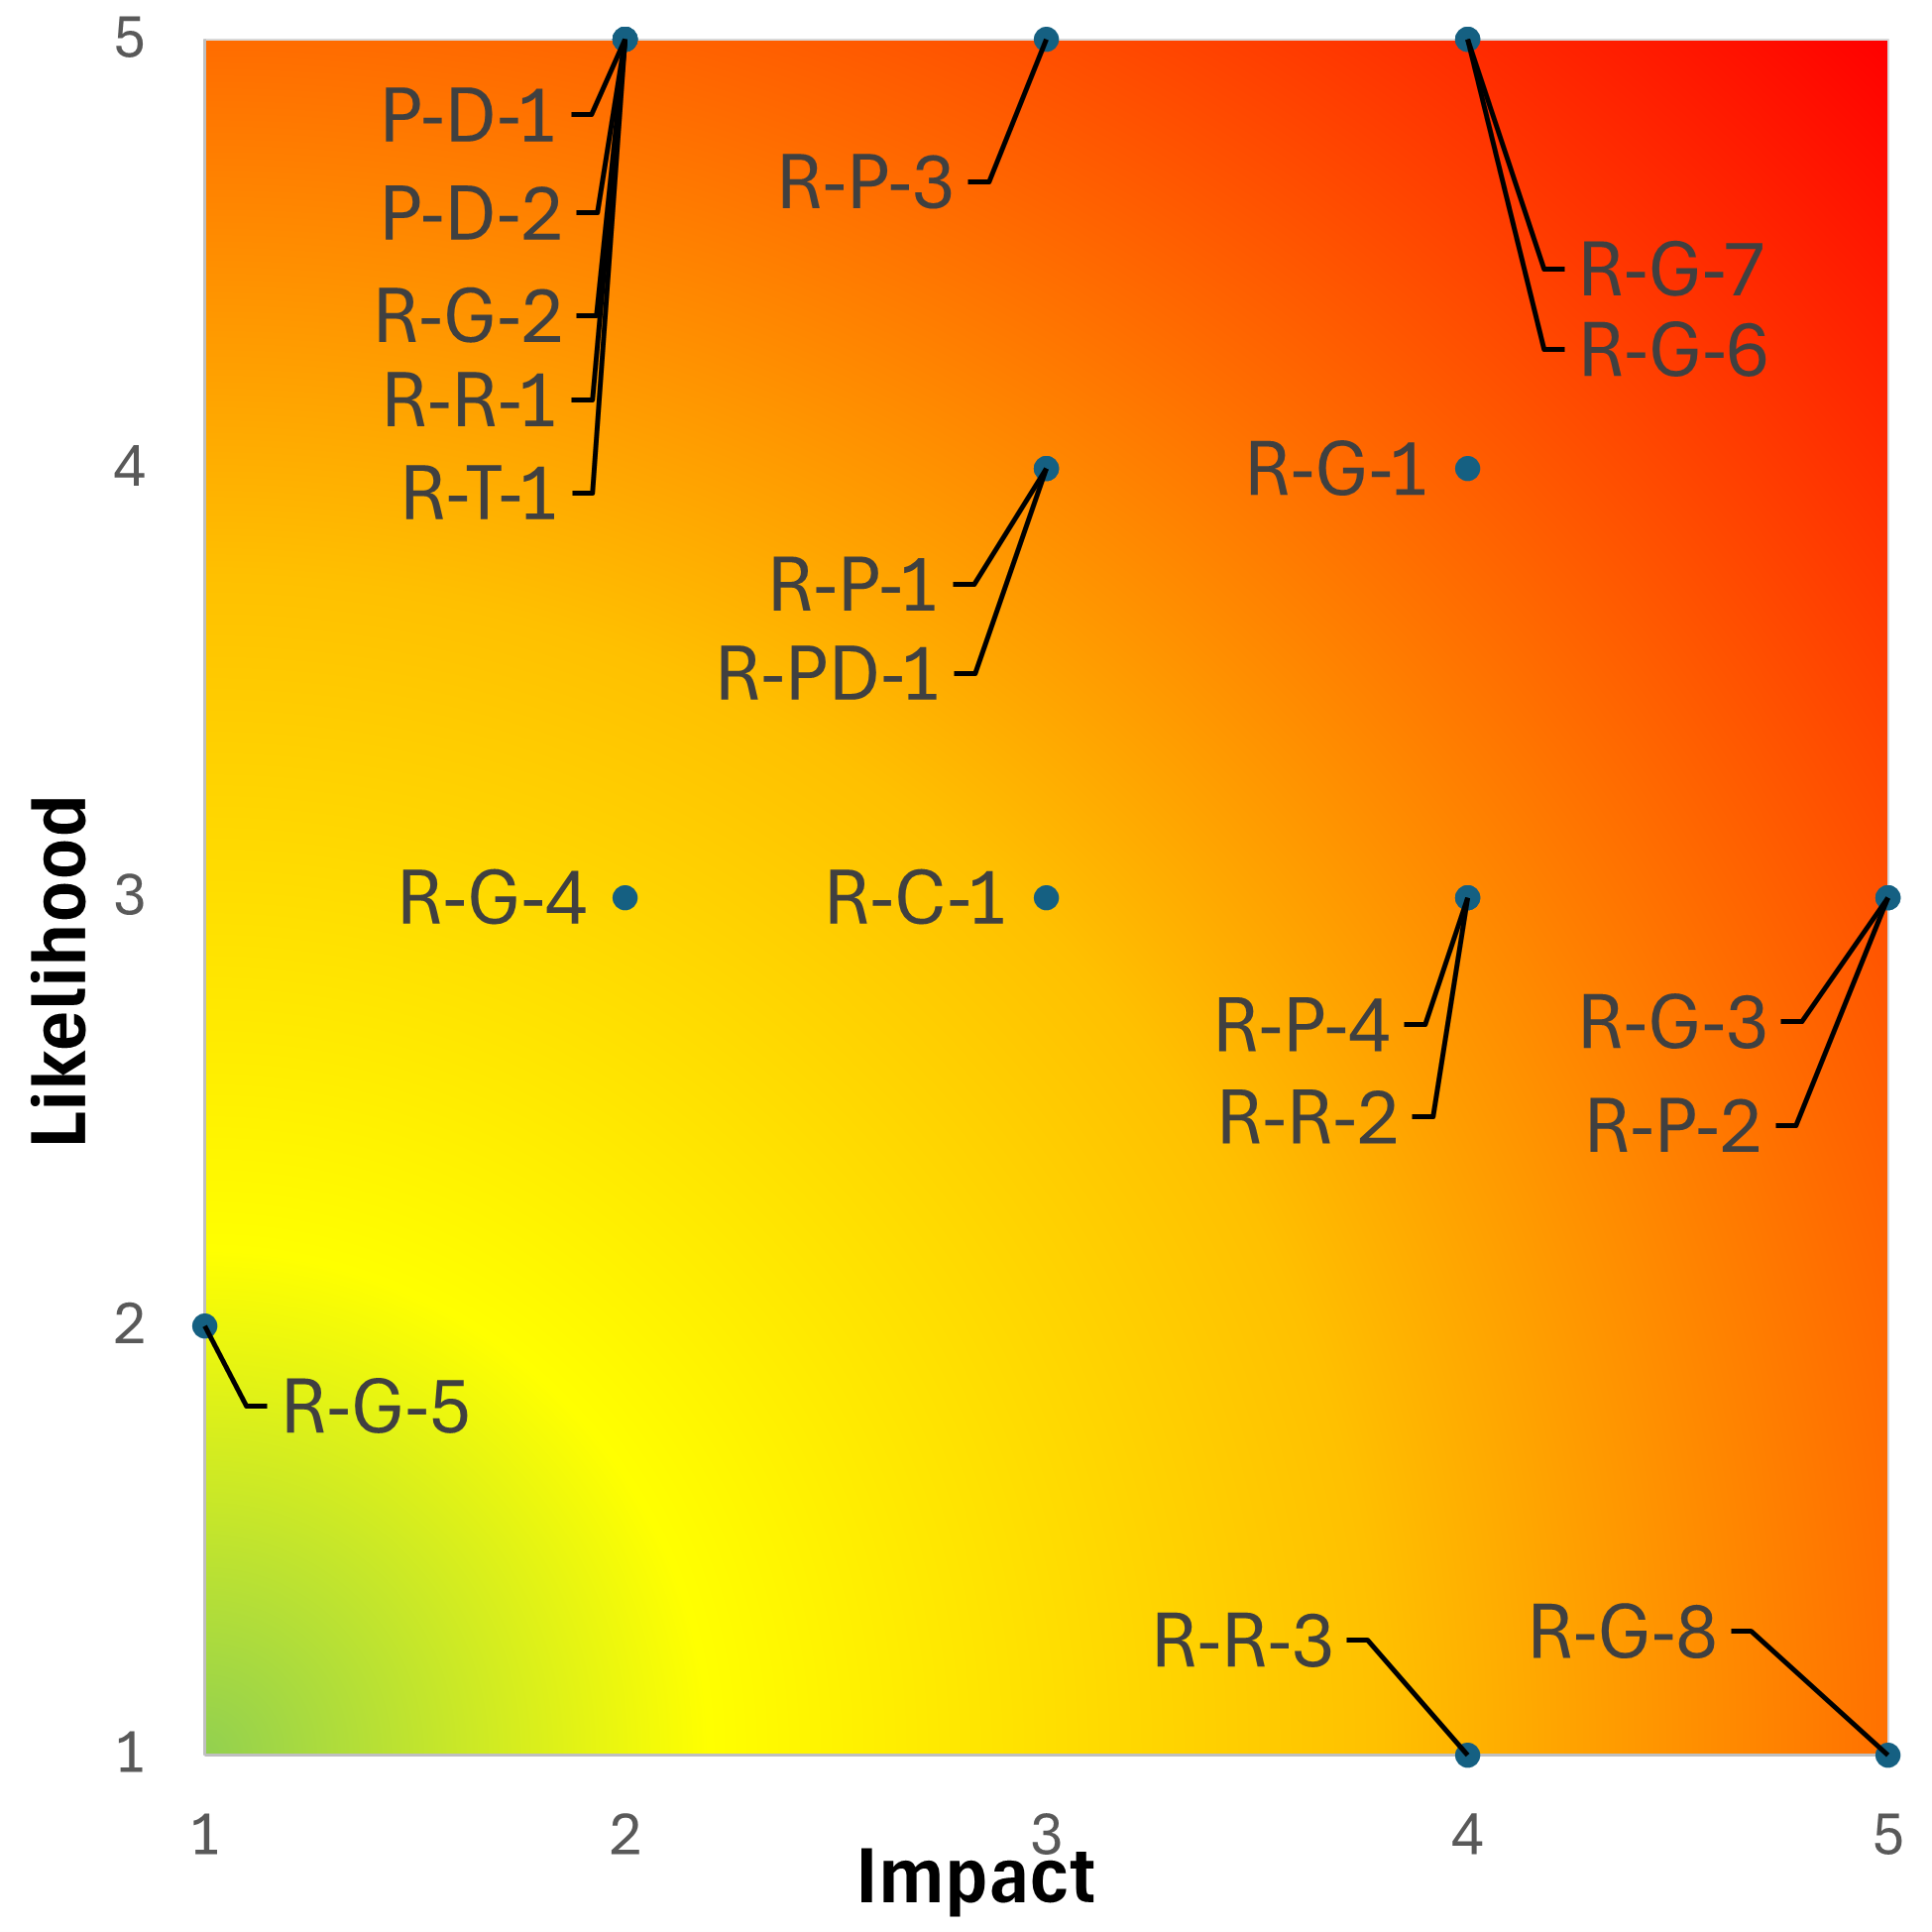
\includegraphics[width=\linewidth]{figures/Risk_map_unmitigated.png}
        \caption{Unmitigated risk map}
        \label{fig:unmitigated}
    \end{subfigure}
    \hspace{0.05\linewidth} % Adjust the spacing between the subfigures
    \begin{subfigure}[b]{0.45\linewidth}
        \centering
        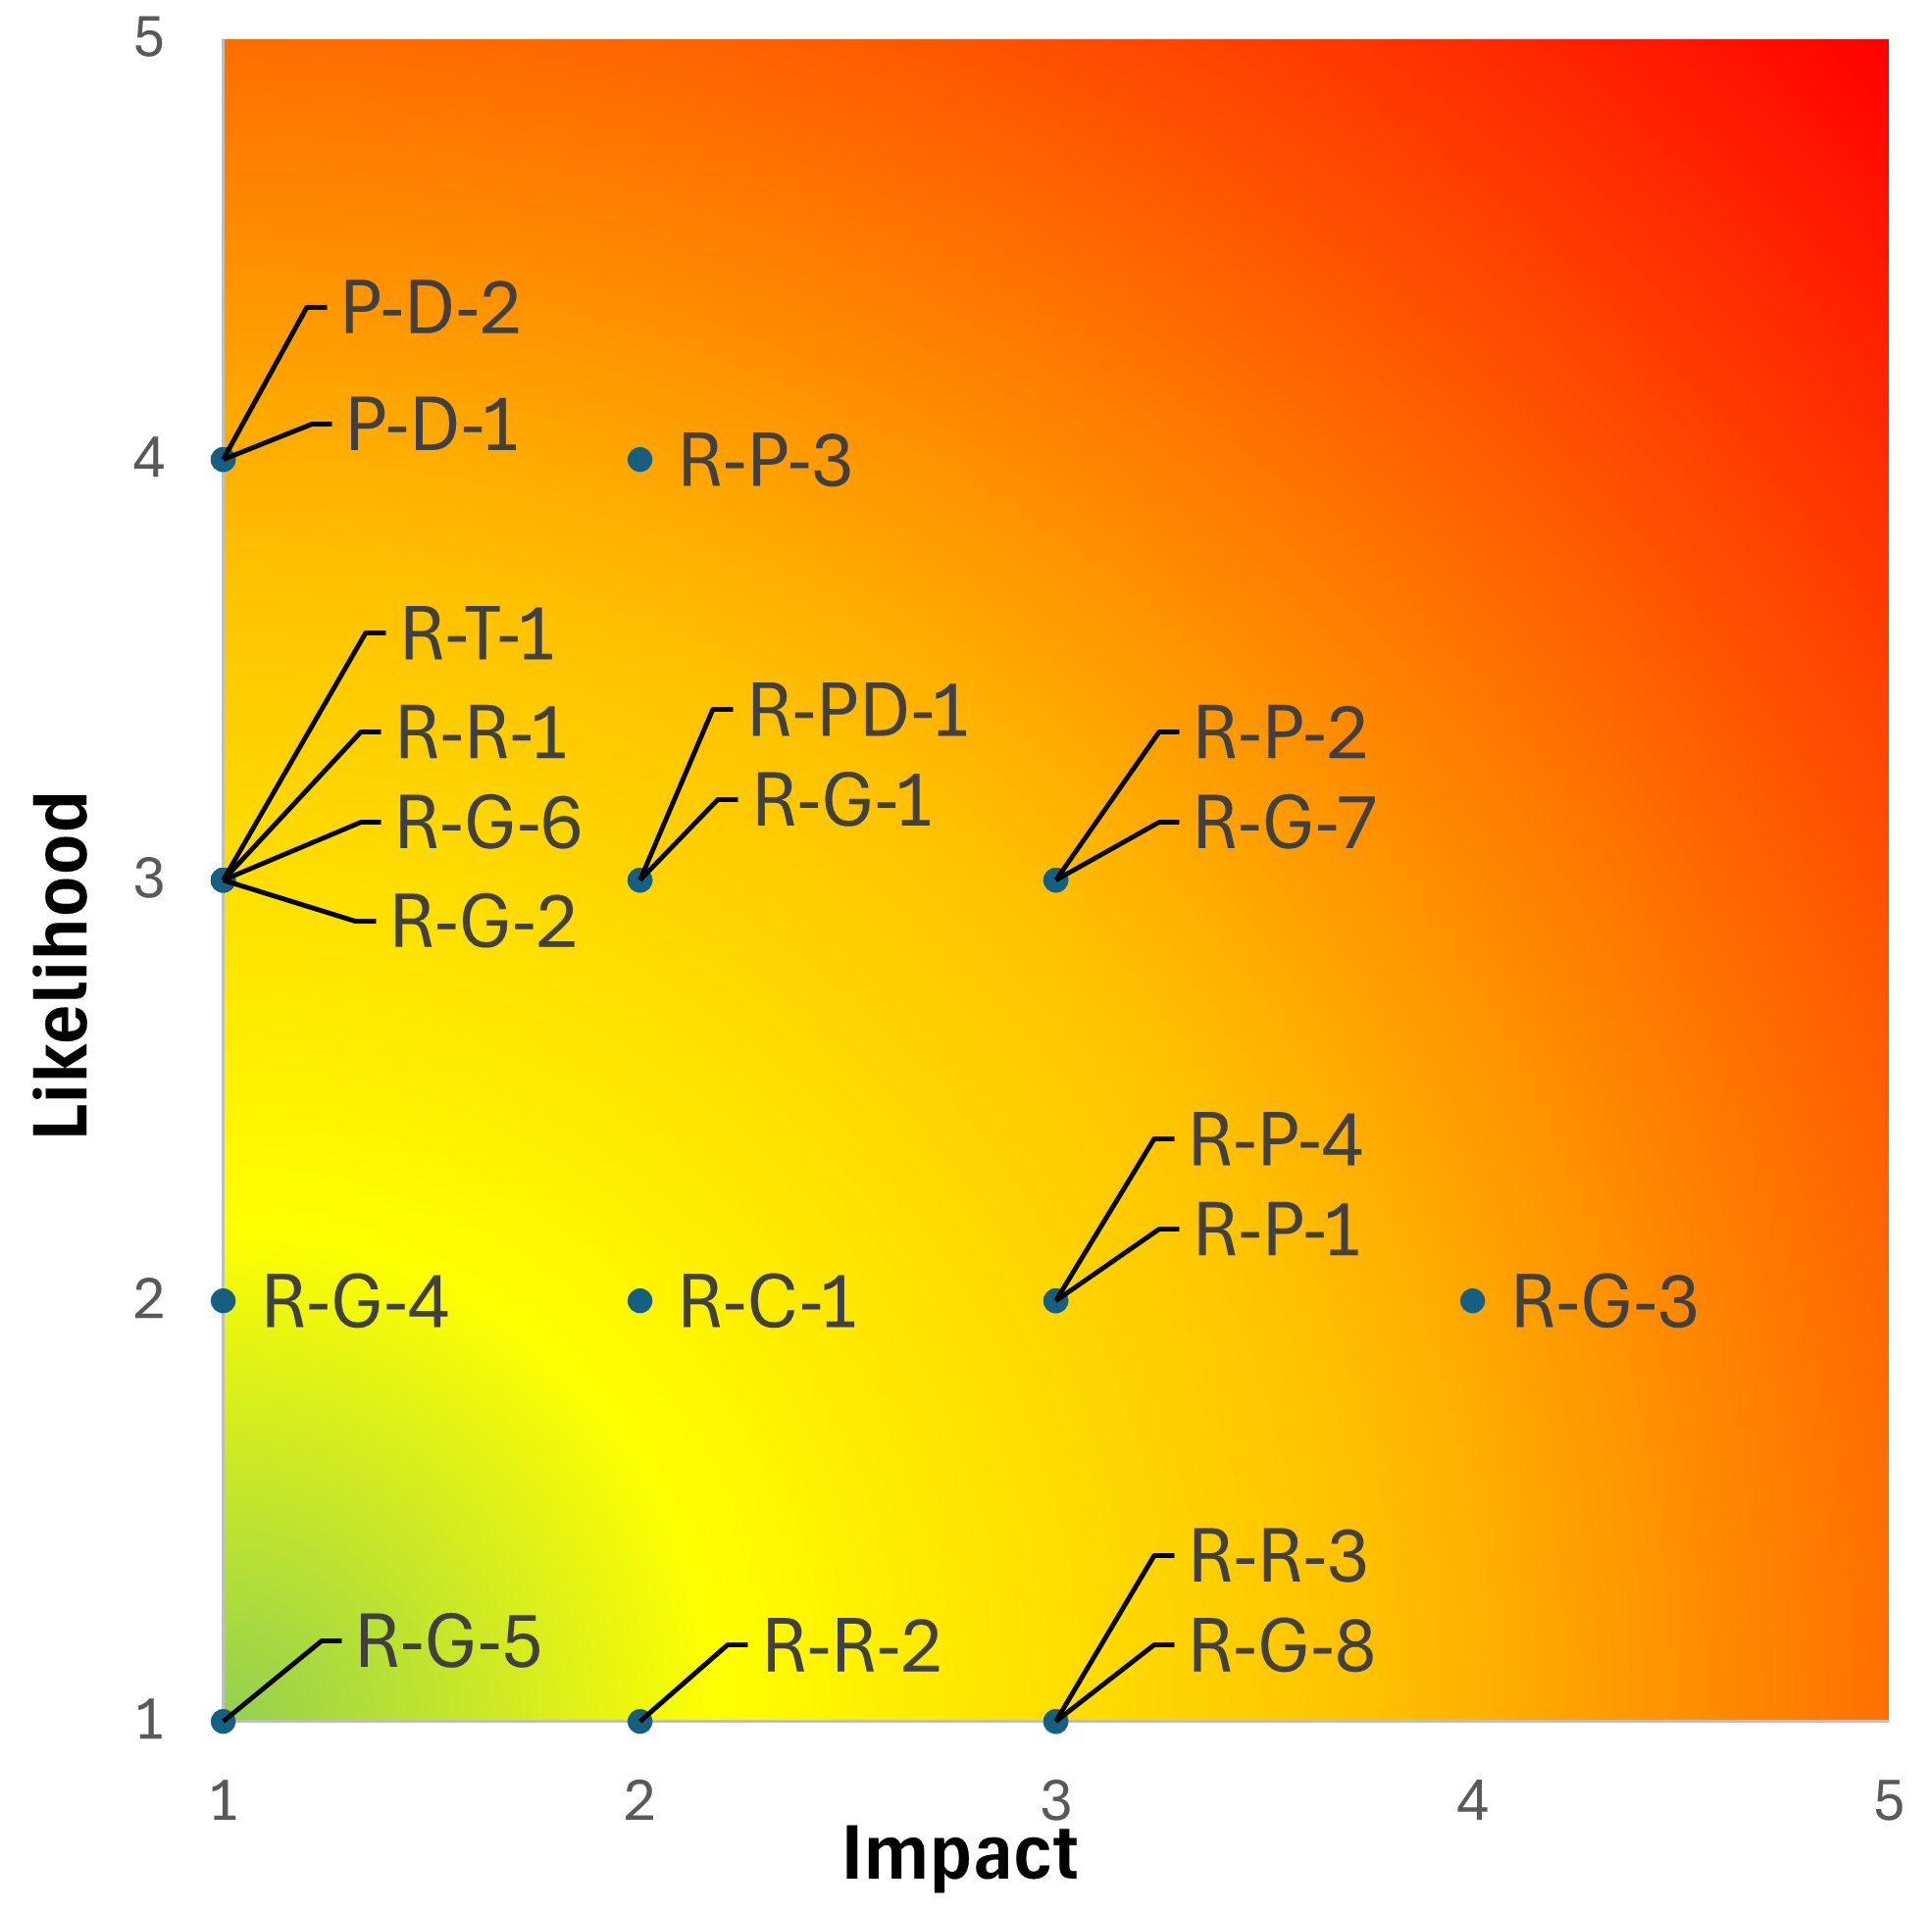
\includegraphics[width=\linewidth]{figures/Risk_map_mitigated.png}
        \caption{Mitigated risk map}
        \label{fig:mitigated}
    \end{subfigure}
    \caption{Comparison of unmitigated and mitigated risk maps}
    \label{fig:riskmaps}
\end{figure}